%-*-coding: utf-8-*-
\chapter{Существующие алгоритмы}

\FloatBarrier

\section{Обзор}

Известны различные алгоритмы поиска мультипутей в графе
\cite{Hyperstar}, \cite{Hyunmyung}, \cite{Dial}. Однако для этих алгоритмов характерны следующие
недостатки: 
\begin{enumerate}
    \item Алгоритмы разрабатывались для других целей. Например, для поиска
      маршрутов по дорогам, на общественном транспорте, когда нужно
      учитывать ожидание транспорта. В то же время при движении по
      воде нет никаких дорог, имеются лишь полигональные препятствия в
      виде суши.
    \item Работая с абстрактными графами, эти алгоритмы не учитывают,
      реальное физическое расположение вершин в графе.
    \item При поиске маршрутов по воде получаются слишком похожие пути.
\end{enumerate}

\FloatBarrier

\section{Adapted Spiess and Florian}

В \cite{Hyperstar} представлено описание похожих алгоритмов поиска
мультипутей. Для примера была предпринята попытка адаптировать ASF
алгоритм для имеющейся задачи. В оригинальном алгоритме каждому ребру
графа соответствует максимальное время ожидания. На основе этих времён
и весов каждому ребру присваивается вероятность быть использованным в
итоговым пути.

Для поиска маршрутов на воде каждому ребру графа сопоставляется
случайное время ожидания, после чего строится распределение
вероятностей. Затем на основе полученного распределения строятся
маршруты, пока не встретится два одинаковых или не наберётся
максимальное число маршрутов.

TODO: про трапецоидную карту, картинки.

\FloatBarrier

\section{Algorithm based on path overlap}

В \cite{Hyunmyung} описывается другой алгоритм поиска мультипутей,
предназначенный для дорожных сетей. Этот алгоритм стремится находить
непохожие пути. TODO: краткое описание алгоритма.

Однако, поскольку при движении по воде нет дорог, то даже не
перекрывающиеся маршруты оказываются очень похожими.

\begin{figure}
    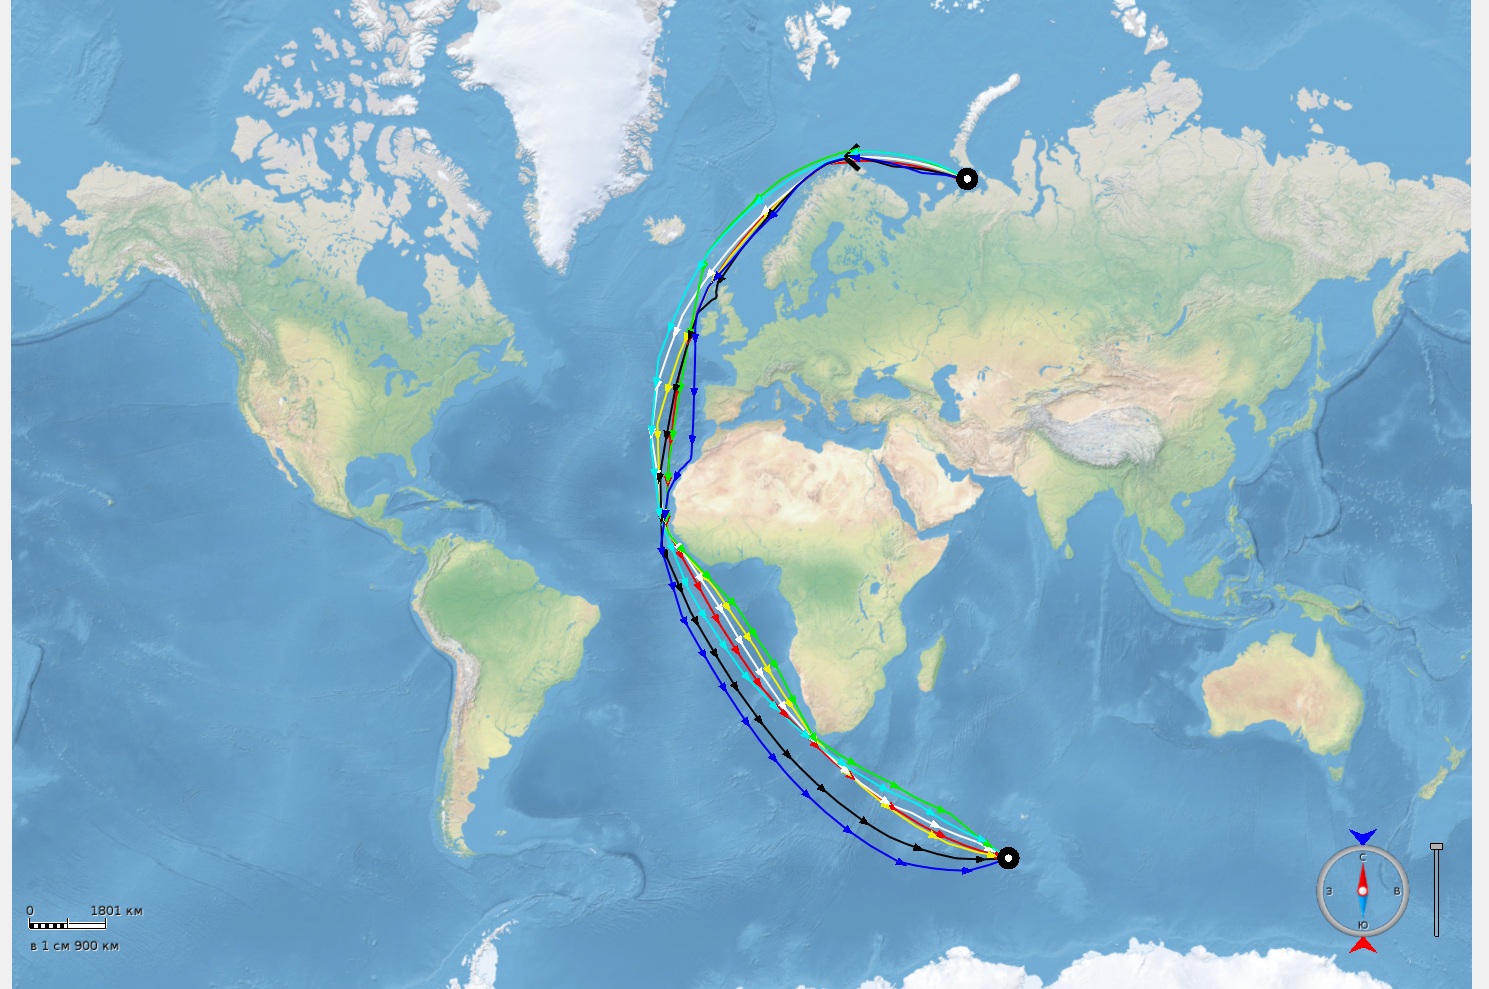
\includegraphics[width=\textwidth]{comparison-with-existing-bad}
    \caption{Пример множества путей, найденного алгоритмом}
\end{figure}

\begin{figure}
    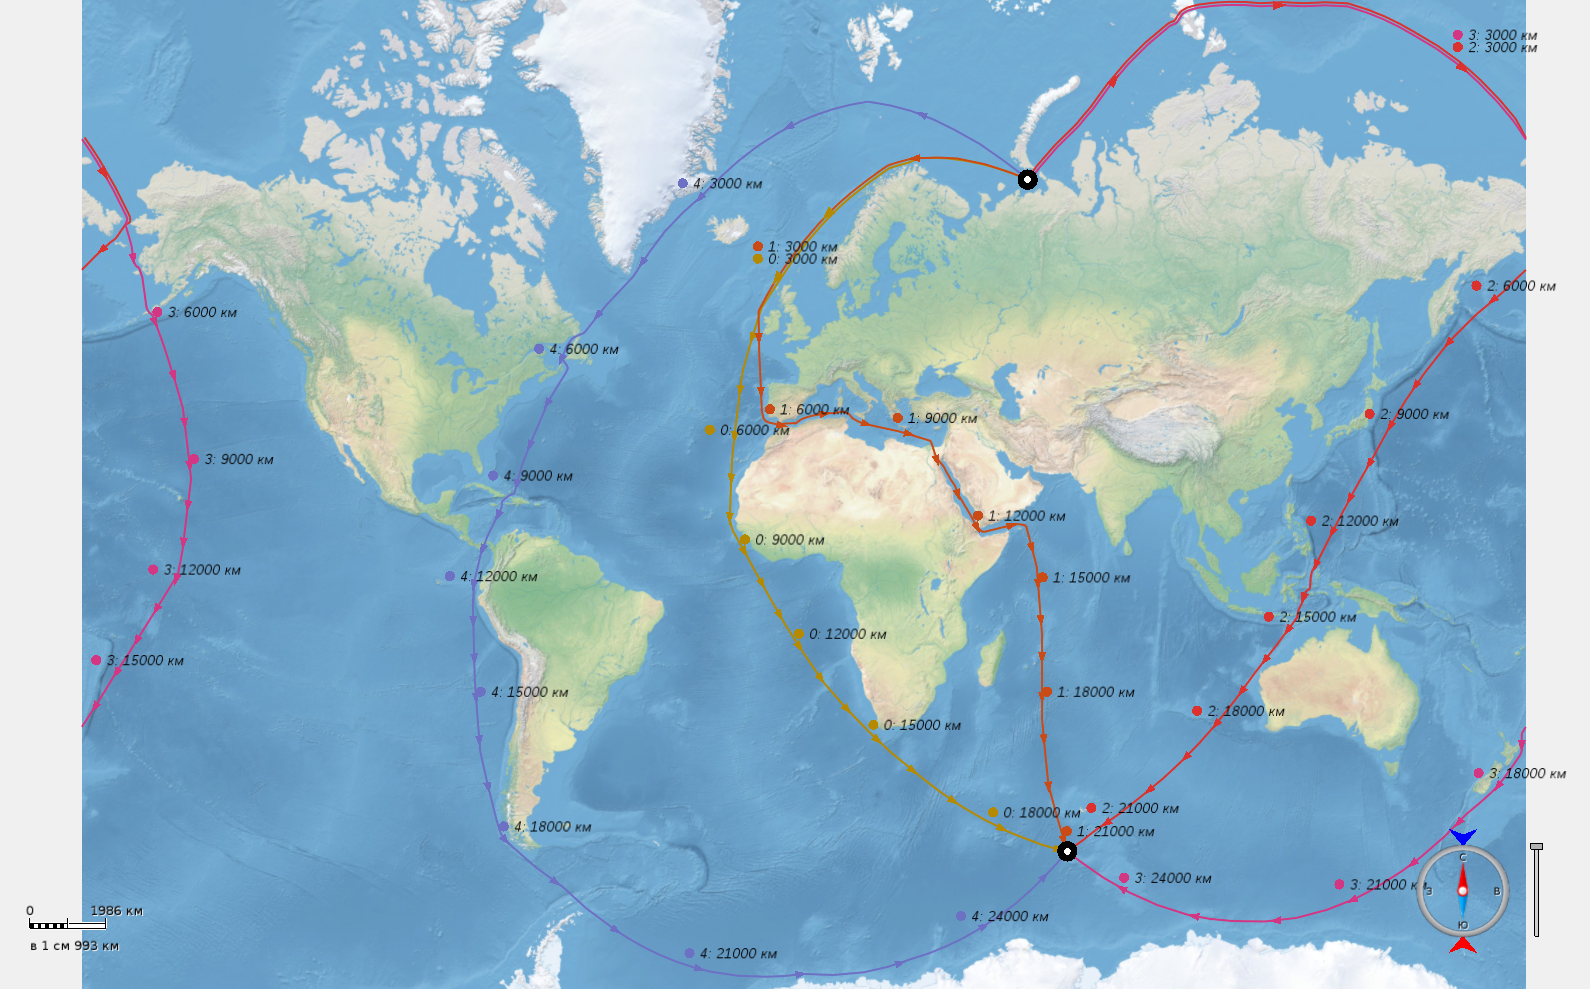
\includegraphics[width=\textwidth]{comparison-with-existing-good}
    \caption{Желаемое семейство маршрутов}
\end{figure}

\FloatBarrier

\section{Dial algorithm}

TODO

\FloatBarrier

